% Created 2019-07-22 Mon 19:06
% Intended LaTeX compiler: pdflatex
\documentclass[11pt]{article}
\usepackage[utf8x]{inputenc}
\usepackage[T1]{fontenc}
\usepackage{graphicx}
\usepackage{grffile}
\usepackage{longtable}
\usepackage{wrapfig}
\usepackage{rotating}
\usepackage[normalem]{ulem}
\usepackage{amsmath}
\usepackage{textcomp}
\usepackage{amssymb}
\usepackage{capt-of}
\usepackage{hyperref}
\setlength\parindent{0pt}
\setlength\parindent{0pt}
\usepackage{placeins}
\usepackage[francais, english]{babel}
\selectlanguage{francais}
\author{Billal Boudjoghra}
\date{\today}
\title{Mémoire}
\hypersetup{
 pdfauthor={Billal Boudjoghra},
 pdftitle={Mémoire},
 pdfkeywords={},
 pdfsubject={},
 pdfcreator={Emacs 26.2 (Org mode 9.1.9)}, 
 pdflang={English}}
\begin{document}

\maketitle
\tableofcontents

\newpage
\section{Sportagraph}
\label{sec:org7859fcd}
Sportagraph est une start-up filiale de Everspeed, fondée en 2013 et lancée en 2016 après trois années de recherche et développement (R\&D).\\
Son produit est un DAM (Digital Asset Manager) spéecialisé dans les événements sportifs.\\

Le DAM permet aux utilisateurs de stocker et de gérer plusieurs types de fichiers (principalement des images, mais les vidéos et d’autres types sont aussi supportés).\\
L’équipe travaillant sur ce projet est composée de :\\
\begin{itemize}
\item Alex Macris : Chief Experience Officer\\
\item Edouard Binchet : Chief Strategy and Operation Officer\\
\item Régis Jean-Gilles : Lead Server Developer (mon tuteur d'alternance)\\
\item Benoit Hozjan : SaaS operation manager\\
\item Francois Jacquier : Lead Developer Front\\
\item Khedidja Almherabet : Développeur front-end\\
\item Mate Gyomrei : Développeur front-end\\
\item Daniel Denke : Développeur iOS\\
\item Zoltan Tarsoly : Test Automation Engineer\\
\item Youva Ammaouche : Assistant chef de projet\\
\item Stéphane : Développeur front-end\\
\item Ashant : Développeur front-end\\
\end{itemize}

En tant que développeur back end, je suis chargé de rajouter de nouvelles fonctionnalitées au DAM.\\
L'une des missions qui m'a été affectée est la détection des replays dans les vidéos de sport.\\
Cette fonctionnalité nous permettra de fournir à nos clients un résumé automatique des vidéos qu'ils publient sur notre plateforme.\\

\newpage
\section{Introduction}
\label{sec:org6699185}
Au cours des dernières années, les techniques d'apprentissage automatique ont joué un rôle de plus en plus important dans les systèmes de reconnaissance automatique.\\
Les avancements dans le domaine de l'apprentissage profond et l'accès à un volume massif de données ont permi de mettre en place des solutions de plus en plus performantes.\\
En particulier, l'adoption globale des téléphones intelligents et de leur caméra intégrée a accru de manière exponentielle le nombre de vidéos disponibles sur Internet, à tel point qu'il est devenu impossible pour l'humain d'ingérer manuellement le contenu de toutes les vidéos disponibles sur la toile.\\
Dans cet étude, nous allons nous intéressons à la tâche de "video summarization" ou, en français, de récapitulation de vidéo.\\
Plus particulièrement, nous focalisons notre recherche sur les vidéos de sport.\\

Dans ces vidéos, notre objectif va être de parvenir à identifier les replays; car à partir de ces replays, nous serons capables de mettre en avant les moments importants du match.\\

\textbf{Pourquoi les replays ?} Un replay est la retransmission d'une action qui s'est déjà passé au cours d'une vidéo.\\
Les replays sont intéressants car ils sont un indicateur d'un moment fort dans une vidéo.\\
En effet, c'est l'équipe technique chargée du montage de la vidéo qui décide ou non de créer un replay pour une action, un replay est une annotation humaine sur une vidéo.\\
Typiquement, un replay sera incrusté dans la vidéo après une action importante comme, par exemple, un but ou un pénaltie.\\

\textbf{Caractéristique des replays} Les replays sont introduits et se terminent par un logo (\cite{Hao_Pan_2002}).\\
Ces logos ont en général une apparence qui se démarque facilement des autres images dans la vidéo.\\
Les replays ne sont pas à confondre avec les ralentis.\\
Les ralentis sont un type particulier de replays où l'action est montrée de nouveau en \emph{slow-motion}, mais tous les replays ne sont pas des ralentis.\\
C'est pourquoi, la vitesse de déplacement des objets dans l'image (pour détecter l'effet de \emph{slow-motion}) n'est pas un bon critère pour la détection de replay.\\

L'objectif de notre recherche est double.\\
Dans un premier temps, nous mettons en place un système de détection de replays en utilisant uniquement les méthodes "classiques" tels que ORB (\cite{Rublee_2011}).\\
Ensuite, nous comparons plusieurs approches d'apprentissage automatique pour la tâche de détection dans les vidéos.\\
Enfin, nous comparons l'efficacité des méthodes de vision par ordinateur "classiques" aux méthodes par apprentissage profond (deep learning).\\

\newpage
\section{Analyse d'image : état de l'art concernant la détection de replay}
\label{sec:org5d6ebdf}
L'un des objectifs de notre recherche est de mettre en place un modèle de détection de replays n'utilisant que des techniques ne faisant pas intervenir d'apprentissage automatique.\\
Ce modèle servira de base de comparaison avec le modèle par apprentissage automatique que nous proposerons par la suite.\\
Afin d'avoir le meilleur modèle, nous avons comparé plusieurs approches.\\

La détection de replays est un domaine de recherche à part entière et les articles sont abondants (\cite{Hao_Pan_2002,Ling_Yu_Duan,Chu_2015,Javed_2019} \ldots{}).\\

\subsection{A Robust Replay Detection}
\label{sec:org39e415f}
Cette approche \cite{xu11_robus_replay_detec_algor_soccer_video} détecte les replays en trouvant les logos dans les vidéo.\\
Les logos sont trouvés grâce à la luminance. Nous savons qu'un logo est présent pendant 0.8 secondes soit 18 frames pour une vidéo de 24 FPS.\\
Tous les frames qui ont obtenu un score supérieur à un certain seuil sont considérés comme des candidats pour être le \emph{logo template}.\\
Le \emph{logo template} est le logo qui représente le mieux les logos dans la vidéo et c'est celui-ci qui va servir de référence pour trouver tous les logos.\\

\subsubsection{Calcul du score de la luminance et filtrage des frames}
\label{sec:org0109f3a}
L'idée est de parcourir toute la vidéo et de calculer pour chaque frame la différence de luminance qu'il y a entre ce frame et les 17 frames précédents.\\
Nous obtenons un score L\(_{\text{i}}\) pour chaque frame i dans la vidéo.\\
Tous les frames dont le score est inférieur à un certain seuil sont écartés, les autres vont servir à trouver le logo template.\\

\subsubsection{Recherche du logo template parmis les frames filtrés}
\label{sec:orge18753a}
Le logo template est le frame qui représente le mieux tous les logos dans la vidéo.\\
Pour déterminer le logo template parmis les frames filtrés, l'algorithme K-means est utilisé pour séparer cet ensemble en deux (K = 2) en fonction de la luminance moyenne des frames.\\
Pour trouver le logo template, nous allons chercher dans le cluster avec le centre de cluster le plus élevé, puis sélection le frame m minimisant la distance avec tous les autres frames du cluster.\\

\begin{figure}[htbp]
\centering
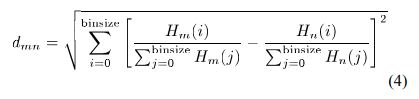
\includegraphics[width=10cm]{robust_calc_dist.JPG}
\caption{Formule de la distance entre deux frames dans le cluster \label{calc-dist}}
\end{figure}


\subsubsection{Recherche des logo}
\label{sec:orga140315}
Une fois que le logo template est déterminé, chaque logo trouvé en précédemment va être comparé avec le logo template.\\
La mesure de comparaison est la distance (figure \ref{calc-dist}) qu'il y a entre le frame et le template dans le cluster.\\
Tous les frames qui ont une distance inférieure à un certain threshold sont considérés comme des logos.\\

\subsubsection{Recherche des replays}
\label{sec:orgfc4aaca}
Une fois que les logos sont détectés, nous pouvons trouver les replays en cherchant les paires de logos éloignés de moins de 80 seconde (durée maximum d'un replay).\\

\subsubsection{Résultats des auteurs}
\label{sec:org7c52c2e}
\section{{\bfseries\sffamily TODO} résultat auteurs pour robust replay}
\label{sec:orga1a0e99}




\subsection{Mean Shift Based video Segment Representation And Applications To Replay Detection}
\label{sec:orga271db2}
Dans cet article \cite{Ling_Yu_Duan}, les auteurs présentent une méthode permettant de détecter les replays.\\
L'idée est d'apprendre une base de représentation compressée de logos avec une méthode comme le spectral hashing (\cite{NIPS2008_3383}), puis de se servir de cette base de données pour trouver les logo au début à la fin de replays.\\
\subsubsection{Algorithme}
\label{sec:orgb02b649}
\begin{verbatim}
L = []
R = []
Segmenter la vidéo en frame
Pour chaque frame f
  Calculer la représentation r_f de f
  Pour chaque représentation r dans la base de représentation:
    Si distance(r_f, r) < Seuil:
      Ajouter f à L
Pour chaque logo l dans L:
  Trouver le logo l' lui correspondant
  Ajouter (l, l') à R
\end{verbatim}
La représentation des images est un hash obtenu par un algorithme de hashing d'image (spectral hashing).\\
La distance utilisée pour comparer le hash des images est la distance de Wasserstein .\\


\subsubsection{Résultats}
\label{sec:org3187a14}
\begin{figure}[htbp]
\centering
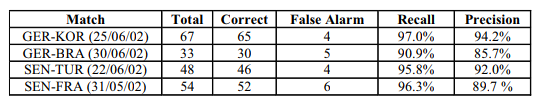
\includegraphics[width=.9\linewidth]{mean_shift_res.png}
\caption{Performance sur la tâche de détection de replay :\label{mean-shift-res}}
\end{figure}
Les résultats obtenus par les auteurs sont présentés dans la Figure \ref{mean-shift-res}.\\
Ceux-ci sont bons, mais l'ensemble de test n'est pas assez représentatif (seulement quatres vidéos).\\
Les avantages des représentations hashées pour les images sont les suivants :\\
\begin{itemize}
\item un hash est compacte (peu d'espace nécessaire pour les stocker)\\
\item comparer des hash est rapide (comparer deux frames)\\
\item chercher un hash dans une table de hachage est rapide (chercher un frame dans une base de données)\\
\end{itemize}
Pour ces raisons, cette approche est tout à fait adaptée à la reconnaissance de logo\\

\newpage
\section{Apprentissage automatique : les bases théoriques}
\label{sec:org59606d4}
Dans notre recherche, nous allons aborder plusieurs types de réseaux d'apprentissage automatique.\\
Nous allons présenter dans cette partie les principes fondamentaux à la bonne compréhension de ces derniers.\\

\subsection{Réseaux de neurones récurrents (RNN)}
\label{sec:orgbc53f65}
Les RNN (Recurrent Neural Networks), ou réseaux de neurones récurrents (RNR) en français, sont capables de répéter leur couche cachée, en utilisant comme entrée la sortie de toutes les couches précédentes et de générer une sortie pour chaque couche.\\
Cela va leur permettre de prendre en entrée des séquences et de retourner des séquences.\\
En effet, pour une entrée [e\(_{\text{1}}\), e\(_{\text{2}}\),\ldots{}, e\(_{\text{n}}\)] et un initialiseur s\(_{\text{0}}\), le RNN va répéter n fois sa couche cachée, de telle sorte à générer une sortie s\(_{\text{1}}\) associée à la couche 1 et à l'entrée (e\(_{\text{1}}\), s\(_{\text{0}}\)); puis il va générer une sortie s\(_{\text{2}}\) associée à la couche 2 et à l'entrée (e\(_{\text{2}}\), s\(_{\text{1}}\)), etc \ldots{}\\
Pour finir, nous aurons en sortie la séquence [s\(_{\text{1}}\), s\(_{\text{2}}\), \ldots{}, s\(_{\text{n}}\)].\\

Par exemple, appliqués à la génération de phrase, les RNN vont être capables de générer (mot par mot, ou n-gram par n-gram) des séquences de phrases de longueur arbitraire.\\

Pour apprendre un modèle, le RNN va avoir besoin d'un ensemble d'entraînement qui met en avant les propriétés qui nous intéressent dans le modèle.\\

La nature récursive de ces réseaux les rend particulièrement adaptés aux tâches de traitement du langage naturel ou pour traiter la temporalité.\\

\subsection{LSTM}
\label{sec:org60194d8}
Les LSTM (Long Short Term Memory) sont un type de RNN \textbf{à portes (gated RNN)}.\\
Ces portes vont permettre de stocker l'information apprise par le réseau à travers le temps.\\
À la différence des RNN classiques, les LSTM sont capables d'oublier de l'information grâce à leur \textbf{leaky unit} afin d'éviter une explosion ou une disparition du gradient.\\
Par exemple, si nous voulons entraîner un LSTM pour qu'il puisse reconnaître une action courte dans une vidéo, ce dernier n'a pas besoin d'enregistrer toutes l'information acquise depuis le premier frame, il lui suffit de connaître un voisinage de quelques frames.\\
La puissance de ces réseaux à portes est que c'est le réseau qui va apprendre à décider quand vider son état interne.\\
Concrétement, cela va leur permettre de pouvoir capturer des dépendances à long terme de manière bien plus efficace que les RNN classiques.\\

\subsection{CNN}
\label{sec:org5697920}
\begin{figure}[htbp]
\centering
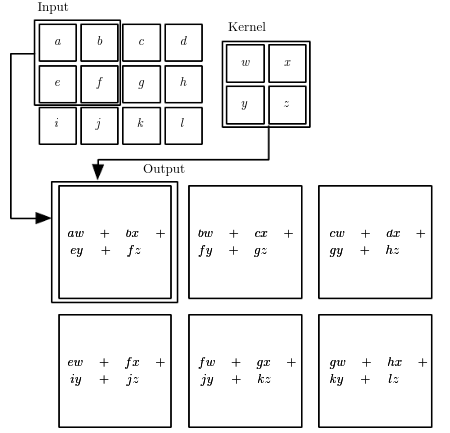
\includegraphics[width=7cm]{convolution.png}
\caption{Opération de convolution \label{convolution}}
\end{figure}
Les CNN (Convolutional Neural Networks), ou réseaux de neurones convolutifs (RNC) en français, sont un type de réseau de neurones qui utilisent la convolution au lieu de la multiplication matricielle dans au moins une de leurs couches.\\
La convolution est une opération qui prend en argument l'entrée (typiquement un vecteur représentant une donnée) et un \textbf{noyau} (les paramètres qui vont être appris par le CNN) et renvoie une \textbf{carte de caractéristiques} (feature map).\\
Le noyau est une matrice qui va parcourir l'entrée et appliquer l'opération de convolution.\\
Pour parcourir l'entrée, celle-ci va être divisée en plusieurs matrices carrées de même taille que le noyau (par exemple 2x2 ou 6x6) en ajoutant si nécessaire du \emph{padding} et du \emph{striding}.\\
La fonction de convolution a trois caractéristiques importantes : l'\textbf{intéraction parcimonieuse} ("sparse interaction"), le \textbf{partage de paramètres} et les \textbf{représentations équivariantes}.\\
La couche de convolution est généralement composée de la fonction de convolution suivie d'une fonction d'activation non linéaire (par exemple, ReLU ou tanh) et d'une d'une fonction de \textbf{pooling}.\\

\subsubsection{Intéraction parcimonieuse}
\label{sec:org75688ae}
\begin{figure}[htbp]
\centering
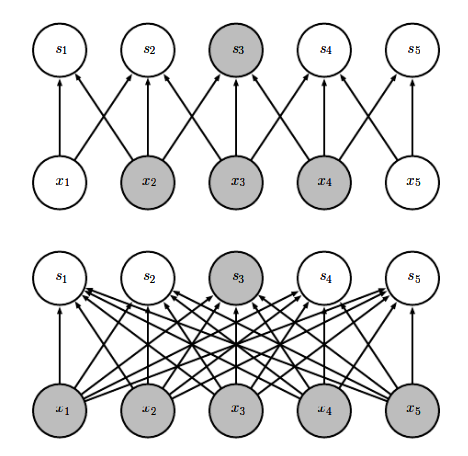
\includegraphics[width=8cm]{sparse_vs_dense.png}
\caption{Intéraction parcimonieuse (en haut), intéraction non parcimonieuse (en bas) \label{sparse-vs-dense}}
\end{figure}

À la différence des réseaux classiques où toutes les sorties intéragissent avec toutes les entrées, les réseaux à convolution ont des \textbf{intéractions parcimonieuses}.\\
C'est à dire que la taille du noyau (donc de l'intéraction avec l'entrée), est plus petite que la taille de l'entrée.\\
Une image a une dimension en entrée de \emph{c*l*w} où \emph{c} est le nombre de canaux de l'image (un seul pour une image en noir et blanc, trois pour une image en couleur), l la largeur en pixel de l'image et w la longueur en pixel de l'image.\\
Une petite image couleur de dimension 100*100 aura 100*100*3 paramètres en entrée, ce qui provoque une explosion combinatoire avec les réseaux classiques qui n'ont pas d'intéraction parcimonieuse car il faudra une connection entre chaque paramètre d'entrée et une entrée du réseau.\\
Un réseau de convolution, quant à lui, aura un noyau d'une dizaine ou d'une centaine de pixel qui parcourt l'image à la recherche de caractéristiques significatives comme des contours.\\
Cela signifie que l'intéraction parcimonieuse permet aux CNN de stocker moins de paramètres que les autres types de réseau.\\
Par conséquent, ils ont donc ont besoin de moins de mémoire (pour la même tâche) et ont une meilleure efficacité statistique.\\
C'est l'une des raisons faisant que les réseaux à convolution sont très efficaces pour le traitement d'image.\\

\subsubsection{Partage de paramètres}
\label{sec:orge98185b}
Dans un réseau classique, un poid (un paramètre) est associé à chaque paramètre d'entrée et ne sert qu'une fois.\\
Tandis que dans un réseau convolutif, le noyau utilisé par une couche de convolution est le même sur toutes les matrices représentant l'entrée.\\
Grâce à ce \textbf{partage des paramètres}, il n'y a que les poids du noyau à apprendre au lieu d'un poid pour chaque neurone d'entrée.\\
De plus, la taille du noyau est en général largement inférieure à celle de la couche d'entrée.\\

\subsubsection{Représentations équivariantes}
\label{sec:orgc22a6d3}
Une fonction est \textbf{équivariante} si, quand l'entrée change, la sortie change de la même manière.\\
En terme mathématique, cela signifique que si \(y = f(x)\) alors \(g(y) = g(f(x))\).\\
Les réseaux convolutifs sont équivariants à la translation.\\
Dans le cas de l'image, celà signifie que le déplacement des pixels n'a pas d'influence sur le réseau.\\

\subsubsection{Pooling}
\label{sec:org302d623}
\begin{figure}[htbp]
\centering
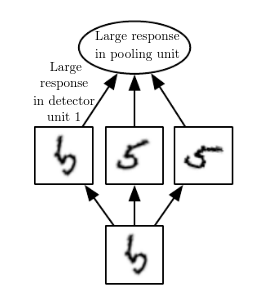
\includegraphics[width=8cm]{pooling.png}
\caption{Pooling \& invariance \label{pooling}}
\end{figure}
La fonction de pooling va modifier la sortie de la couche de convolution.\\
Pour chaque valeur dans la carte des caractéristiques à la sortie de la convolution (après la fonction d'activation), la fonction de pooling va remplacer celle-ci en fonction de la valeur des cases voisines dans la carte.\\
Une fonction de pooling usuelle est max pooling, qui va renvoyer la plus grande valeur dans un voisinage rectangulaire.\\
L'utilité de la fonction de pooling est de rendre la représentation apprise par la couche de convolution \textbf{invariante} à de petites modifications sur l'entrée.\\
Par exemple, dans le cas de la reconnaissance d'image, le réseau ne va pas chercher dans l'image en entrée les informations au pixel près.\\
Si le réseau a appris à détecter les visages, il n'a pas besoin de retrouver l'emplacement des yeux au pixel près, une position approximative de ceux-ci lui suffira.\\
Une autre utilité du pooling est de réduire la taille de la sortie de la couche de convolution.\\
Nous pouvons voir le pooling comme un résumé de la carte des caractéristiques obtenue par convolution.\\

\newpage
\section{Apprentissage profond : état de l'art pour la reconnaissance d'action dans les vidéos}
\label{sec:org902afaf}
Nous nous intéressons à l'état de l'art concernant la détection d'action dans les vidéos.\\
En effet, la transition d'un logo s'effectue sur plusieurs frames consécutifs; il y a donc une composante temporelle à notre recherche, et nous pouvons considérer la transition d'un logo comme une action.\\

\subsection{Two-Stream Convolutional Networks for Action Recognition in Videos}
\label{sec:org5bf81e1}
Cet article est écrit par Karen Simonyan et Andrew Zisserman \cite{DBLP:journals/corr/SimonyanZ14}. Dans celui-ci, ils proposent de séparer la tâche de reconnaissance d'action dans les vidéos en deux parties : une composante spatiale et une composante temporelle.\\

La composante spatiale contient l'information concernant les objets dans la vidéo; tandis que la composante temporelle l'information sur les déplacements de ces objets et de la caméra.\\
A partir de ces observations, les auteurs proposent d'entraîner un classifieur spatial (Spatial stream ConvNet) et un classifieur temporel (Temporal stream ConvNet).\\

Ces classifieurs sont des réseaux de neurones convolutifs profonds.\\

\subsubsection{Classifieur spatial}
\label{sec:orgf18a043}
Ce réseau a une architecture de classifieur d'image classique.\\
Il va permettre de donner un indice fort pour la prédiction, car certaines actions sont très liées à certains objets.\\
De plus, la recherche dans le domaine de la classification est un domaine à part entière; toutes les avancées dans le domaine augmenteront l'efficacité de ce classifieur.\\
Il n'est pas nécessaire d'apprendre ce réseau "from scratch" (de zéro), les approches par transfer learning sont efficaces.\\

\subsubsection{Classifieur temporel}
\label{sec:org834a790}
\begin{figure}[htbp]
\centering
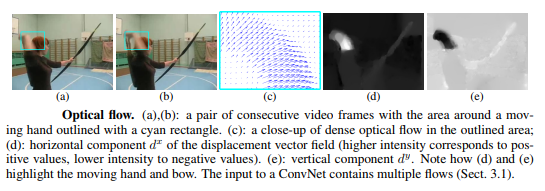
\includegraphics[width=12cm]{optical_flow.png}
\caption{Flux optique \label{optical-flow} \label{opt-flow}}
\end{figure}
L'innovation de l'article vient de l'introduction du classifieur temporel.\\

L'idée est de détecter le mouvement des objets dans la vidéo, car un mouvement est la représentation d'un objet dans le temps.\\
Les auteurs appellent leur approche "optical flow stacking" (empilement de flux optique).\\

Dans celle-ci, ils utilisent la méthode "optical flow" pour détecter le mouvement des objets entre des frames consécutifs.\\

Ils définissent aussi un hyperparamètre L qui définit la distance maximum entre deux frames pour laquel il faut calculer le flux optique.\\
Par exemple, si L=5, alors pour le frame t, il faudra calculer le flux entre le frame t et le frame t+1; entre t+1 et t+2; etc\ldots{} jusqu'à t+4 et t+5.\\
Ainsi, des images représentant le flux optique entre les différents frames de la vidéo vont être générées.\\

Chacunes de ces images servira d'entrée au CNN (classifieur temporel).\\
\subsubsection{Méthode d'évalutation et résultats obtenus}
\label{sec:orgd1fee39}
\begin{figure}[htbp]
\centering
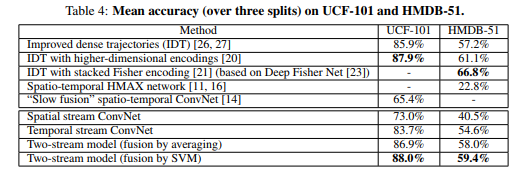
\includegraphics[width=13cm]{two_stream_res.png}
\caption{Résultats obtenus par l'approche Two-stream model \label{two-stream-res}}
\end{figure}

Le classifieur spatial est pré-entrainé avec ImageNet, tandis que le temporel est entraîné de zéro (car il n'y a pas de réseau déjà entraîné pour cette tâche).\\
Les dataset utilisés pour l'entraînement et l'évaluation sont UCF-101 et HMDB-51, contenant à eux deux près de 20000 vidéos annotées.\\

\textbf{Note} Pour calculer la classe d'un frame à l'instant t, les auteurs proposent deux méthodes :\\
\begin{itemize}
\item fusion par la moyenne (by averaging) : y\(_{\text{t}}\) = y\(_{\text{t}}\)\(_{\text{spatial}}\) + y\(_{\text{t}}\)\(_{\text{temporal}}\) / 2\\
\item fusion par SVM (by SVM) : un SVM multiclasse linéaire est entrainé pour prédire la classe à partir du softmax des scores L2-normalisés.\\
\end{itemize}

Les résultats (figure \ref{two-stream-res}) montrent l'efficacité de leur méthode par rapport aux autres approches état de l'art.\\

Nous pouvons voir que leur approche two-stream avec fusion SVM est la plus efficace sur le dataset UCF-101, et qu'elle a aussi de bons résultats sur HMDB-51.\\

Ce qui est le plus intéressant dans cet article, c'est l'amélioration qu'apporte l'ajout de la composante temporelle.\\
En effet, le classifieur d'image simple (spatial) n'a que 73.0\% (UCF-101) et 40.5\% (HMBD-51), tandis que le classifieur qui prend en compte l'image et la temporalité (two-stream model) atteint \textbf{88.0\%} et 59.4\%; ce qui est une nette amélioration.\\

Cet article nous a renforcé dans l'hypothèse qu'il est nécessaire d'étudier une vidéo non pas comme une suite d'images indépendantes, mais comme une suite de séquence avec un lien entre chaque élément de la séquence. La temporalité a une très grande importance pour l'analyse de vidéos.\\

\subsection{Learning Spatiotemporal Features with 3D Convolutional Networks}
\label{sec:org78282ed}
Dans cet article \cite{Tran_2015}, les auteurs proposent une approche pour apprendre les caractéristiques spatio-temporelles dans les vidéos grâce à un réseau de neurones à convolution.\\

Ils font l'hypothése qu'un réseau avec une couche de convolution 3D qui prend en entrée une séquence d'images est capable d'apprendre efficacement les mouvements des objets dans les vidéos.\\

L'objectif est d'apprendre des caractéristiques qui soient :\\
\begin{itemize}
\item génériques : c'est à dire la capacité à représenter différents types de vidéos\\
\item compactes : afin de pouvoir stocker un grand nombre de ces caractéristiques\\
\item efficace (computationnellement): pour traiter les vidéos en temps réel\\
\item simples : afin de fonctionner même avec les modèles simples (comme un classifieur linéaire)\\
\end{itemize}

\subsubsection{C3D: Convolution et pooling 3D}
\label{sec:org07a257d}
\begin{figure}[htbp]
\centering
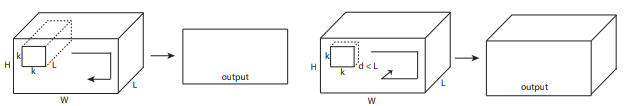
\includegraphics[width=.9\linewidth]{c3d_idea.png}
\caption{Convolution 2D sur une séquence d'images (gauche), convolution 3D sur une séquence d'images (droite) \label{c3d-idea}}
\end{figure}
Les auteurs appellent leur approche C3D (3D ConvNet).\\
Comparé aux réseaux à convolution 2D, C3D est capable de modéliser plus efficacement l'information spatio-temporelle grâce à la convolution et au pooling sur trois dimensions.\\
La convolution 2D appliquée à une image produira en sortie une image, la convolution 2D appliquée à une suite d'images produira aussi une image.\\
C'est pourquoi les réseaux à convolution 2D perdent l'information temporelle après l'opération de convolution. La convolution 3D permet, elle, de préserver cette information.\\


\subsubsection{Architecture et entraînement du réseau}
\label{sec:org57a0589}
\begin{figure}[htbp]
\centering
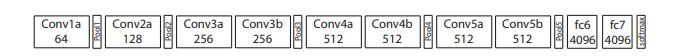
\includegraphics[width=13cm]{c3d_architecture.jpg}
\caption{Architecture C3D \label{arch-c3d}}
\end{figure}
L'entrée de ce réseau est de dimension c * l * h * w où c est le nombre de canaux des images (3 pour la couleur, 1 pour les images en noir et blanc), l le nombre d'images dans les séquences, h la longueur et w la largeur en pixel des images.\\

L'architecture conseillée par les auteurs est 8 couches de convolution et 5 couches de pooling, ainsi que 2 couches complètement connectées et la fonction softmax pour la couche de sortie.\\
Le kernel recommandé par les auteurs est 3 * 3 * 3 avec un pas (stride) de 1 * 1 * 1 pour toutes les couches de convolution.\\
Toutes les couches de pooling sont max pooling avec une taille de kernel 2 * 2 * 2 (sauf pour la première qui est 1 * 2 * 2) avec un stride 2 * 2 * 2 (sauf pour la première qui a un stride de 1 * 2 * 2).\\
Pour finir avec l'architecture, les deux couches complètement connectées ont 4096 sorties.\\

Ce réseau va être entraîné de zéro par descente du gradient à partir de séquences d'images annotées.\\
Le taux d'apprentissage est de 0.003 et est divisé par 10 toutes les 4 epoch.\\
L'entraînement s'arrête après 16 epoch.\\

Après l'entraînement, le réseau peut être utilisé comme un extracteur de caractéristiques pour des tâches d'analyse vidéo.\\
Pour se faire, la vidéo va être découpée en des clips de 16 frames (avec 8 frames de chevauchement entre deux clips consécutifs).\\
Ensuite, chacun de ces clips va être passés au réseau et l'avant dernière couche complètement connectée (fc6) va contenir les caractéristiques du clip.\\

\textbf{Qu'est-ce que ce réseau apprend ?} Ce réseau apprend à se focaliser sur l'image des premiers frames, et à traquer leur déplacement dans les frames suivants.\\

\subsubsection{Résultat pour la tâche de reconnaissance d'action}
\label{sec:orgcfc3657}
\begin{figure}[htbp]
\centering
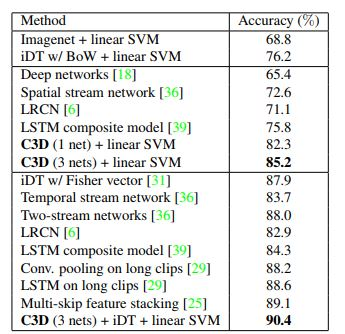
\includegraphics[width=7cm]{c3d_result.jpg}
\caption{Résultats pour l'approche Learning Spatiotemporal Features with 3D Convolutional Networks (C3D) comparés à d'autres approches état de l'art \label{c3d-res}}
\end{figure}
Ces résultats (figure \ref{c3d-res}) ont été obtenus par les auteurs pour la tâche de reconnaissance d'action sur le corpus de vidéo UCF101.\\
Nous voyons que l'approche par réseau à convolution 3D est la plus efficace.\\

\subsubsection{Conclusion}
\label{sec:org12268f9}
Dans cet article, les auteurs ont adressé le problème de la temporalité dans les vidéos.\\
Ils ont montré qu'un réseau à convolution 3D est capable de modéliser l'information temporelle et spatiale simultanément, et donc d'obtenir de meilleurs résultats que les réseaux à convolution 2D sur plusieurs tâches d'analyse de vidéos.\\
De plus, cette approche est très élégante car elle fonctionne sans ajout artificiel de caractéristiques (comme le flux optique), c'est le réseau qui va se charger d'apprendre ce dont il a besoin pour apprendre la temporalité.\\

\subsection{Beyond Short Snippets: Deep Networks for Video Classification}
\label{sec:orgbbfc719}
Dans cet article \cite{Joe_Yue_Hei_Ng_2015}, les auteurs proposent d'utiliser une architecture hybride à base de CNN et de RNN (LSTM) pour l'analyse vidéo.\\
Leur objectif est d'apprendre des dépendances à long terme dans les vidéos, d'où l'utilisation d'un LSTM.\\
Les CNN sont des réseaux particulièrement efficaces pour analyser les frames des vidéos, c'est le CNN qui va se charger de la composante spatiale de la vidéo.\\
Les LSTM va servir à apprendre la composante temporelle.\\

\subsubsection{Approche}
\label{sec:org3d48e34}
L'objectif des auteurs est d'apprendre des dépendances à long terme dans les vidéos.\\
Les réseaux à convolution sont très efficaces pour l'analyse d'image; mais leur coût computationnel est très élevé.\\
C'est pourquoi, il n'est pas possible de se servir d'un CNN pour apprendre les dépendances à long terme; en effet, il faudrait que le réseau prenne en entrée toute la vidéo (ou bien une grande partie), ce qui n'est pas possible avec la puissance de calcul actuelle.\\
Les auteurs font l'hypothèse que tous les frames dans la vidéo ne sont pas utiles, et qu'il est judicieux de ne garder qu'un sous-ensemble des frames de la vidéo; ils proposent donc de ne traiter qu'un frame par seconde. L'intérêt de ne garder qu'un sous ensemble des images de la vidéo et qu'il va donc être possible de traiter la vidéo sur une plage temporelle plus large pour le même coût en calcul.\\
Néanmoins, ne regarder qu'une seule image par seconde dans la vidéo ne préserve pas le déplacement des pixels entre l'instant t et l'instant t + 1 (en seconde) et donc l'information du mouvement des objets.\\
Pour palier à ce problème, le flux optique (de la même manière que \cite{DBLP:journals/corr/SimonyanZ14}) est calculé entre les frames adjacents.\\
Ainsi, l'information temporelle et l'information spatialle sont préservées, tout en ne traitant qu'une seule image par seconde, ce qui réduit beaucoup le coût de calcul.\\
Pour apprendre les dépendances qu'il y a entre les frames, un LSTM est utilisé; celui-ci va traiter les vidéo comme des séquences d'images et va apprendre à prédire la classe de la vidéo en fonction de ces séquences.\\
\subsubsection{Architecture}
\label{sec:orgdf9e2d2}
\begin{figure}[htbp]
\centering
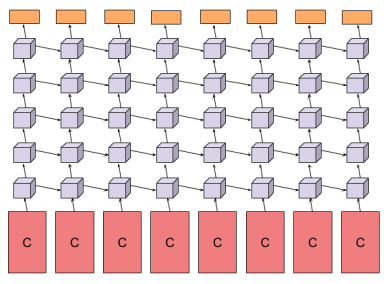
\includegraphics[width=8cm]{cnn_lstm.PNG}
\caption{Architecture du LSTM \label{arch-lstm}}
\end{figure}
Comme pour \cite{DBLP:journals/corr/SimonyanZ14}, un réseau à convolution va être utiliser pour extraire les caractéristiques visuelles de la vidéo.\\
Les architectures utilisées pour ce réseau sont GoogLeNet et AlexNet.\\

L'architecture proposée pour le LSTM est présentée en \ref{arch-lstm}.\\
La sortie du CNN est processée par propagation avant à travers cinq couches de LSTM.\\
La couche de sortie du LSTM est munie de la fonction softmax et prédit une classe à chaque étape.\\
Les paramètres du réseau à convolution et de la couche de sortie du LSTM sont partagés pour toutes les étapes.\\

\subsubsection{Utilisation du flux optique}
\label{sec:orgf130264}
Le flux optique encode l'information des déplacements des objets dans la vidéo.\\
Comme pour l'approche \cite{DBLP:journals/corr/SimonyanZ14}, les images de flux vont être pré-calculées et servir lors de l'entrainement du CNN.\\

\subsubsection{Résultat obtenu}
\label{sec:org4f43fa7}
\begin{figure}[htbp]
\centering
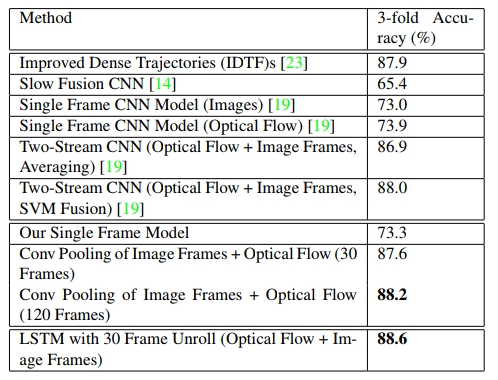
\includegraphics[width=10cm]{cnn_lstm_res.png}
\caption{Résultat obtenu pour l'approche combinant CNN et LSTM (LSTM with 30 Frame Unroll) \label{cnn_lstm}}
\end{figure}
Les auteurs évaluent leur approche sur le dataset Sports-1M et UCF-101 sur la tâche de classification de vidéos.\\
Nous pouvons voir que leur approche obtient les meilleurs résultats (88.6\% contre 88.0\% pour \cite{DBLP:journals/corr/SimonyanZ14}).\\
Ces résultats sont intéressants car à la différence des autres approches, celle-ci est capable de prédire une classe pour des morceaux de vidéos pouvant aller jusqu'à deux minutes (contre quelques secondes pour les autres).\\
De plus, les meilleurs résultats sont là aussi obtenus en utilisant le flux optique, confirmant l'hypothèse faite par \cite{DBLP:journals/corr/SimonyanZ14} que ce dernier est nécessaire pour le traitement des vidéos.\\

Dans notre cas, cette approche n'est pas la plus adaptée. En effet, nous souhaitons reconnaitre les logos dans les vidéos, or un logo ne dure pas plus longtemps que quelques secondes et les dépendances à long-terme que le LSTM va apprendre ne nous intéressent pas.\\
Néanmoins, une variante de celle-ci où le LSTM reçoit en entrée une séquence de frames consécutifs (et pas une séquence formée d'un frame par seconde) pourrait avoir de bons résultats pour la tâche de détection de logos.\\

\newpage
\section{Les approches proposées}
\label{sec:orgd5a30ed}
L'objectif de notre recherche est de détecter les replays dans les vidéos de sport\\

Pour détecter les replays, nous faisons les hypothèses suivantes :\\
\begin{itemize}
\item un replay a un logo de début (I)\\
\item un replay a un logo de fin (II)\\
\item les logos de début et de fin sont les mêmes (III)\\
\item les logos ont une forme facilement reconnaissable qui se distingue des  autres images dans la vidéo (IV)\\
\item un replay dure entre 2 et 90 secondes (V)\\
\end{itemize}

Nous proposons plusieurs approches permettant de détecter les logos de replay dans les vidéos de sport.\\
En premier lieu, nous proposons deux approches n'utilisant que des algorithmes d'analyse d'images classiques (flouttage, filtre de Canny, ORB, \ldots{}) :\\
\begin{itemize}
\item la première se sert de l'algorithme ORB (\cite{Rublee_2011}) et de l'algorithme K-Means\\
\item la seconde utilise la détection de contours pour trouver les images avec des contours similaires dans la vidéo\\
\end{itemize}
Ensuite, nous présentons deux approches par apprentissage profond :\\
\begin{itemize}
\item la première utilise un réseau à convolution 3D sur une séquence d'images (similaire à \cite{Tran_2015})\\
\item la seconde utilise un réseau à convolution 2D sur des images représentant le flux optique des objets dans la vidéo\\
\end{itemize}

\subsection{Détection des plans}
\label{sec:org933e647}
Les approches que nous proposons itérent sur tous les frames de la vidéo, à la recherche des logo pouvant se trouver au début et à la fin des replays.\\
Si nous faisons l'hypothèse qu'un replay entraînera toujours un changement de plan, alors au lieu de rechercher les logos parmi tous les frames de la vidéo, nous pouvons réduire la recherche à tous les frames qui sont entre deux plans.\\

C'est pourquoi nous allons chercher une méthode permettant de détecter les changements de plan dans les vidéos.\\

\subsubsection{Online, Simultaneous Shot Boundary Detection And Key Frame Extraction For Sports Videos Using Rank Tracing}
\label{sec:org9ff91a1}
Cette méthode est proposée par W. Abd-Almageed en 2008 \cite{Abd_Almageed_2008}.\\

Chaque frame est converti en HSV et les histogrammes H, S et V sont calculés.\\
Un vecteur est formé pour chaque frame à partir de ces histogrammes.\\
Ensuite, une matrice M de dimension N * L, représentant une fenêtre de N frames va être formée à partir de ces vecteurs, où L est la taille des histogrammes et N la taille de la fenêtre.\\

L'algorithme SVD (singular value decomposition) va être appliqué sur M.  \(M = UWV\), où W est la matrice de valeurs singulières.\\

Les diagonales de la matrice W comportent des poids S ordonnés de manière non croissante.\\
Le premier poid S\(_{\text{1}}\) est le poid maximal. Ces poids représentent l'information contenue dans le vecteur V.\\

Nous allons assigner un rang à la matrice M,  ce rang va être égal au nombre d'éléments s dans S tel que s/S1 > threshold. Le rang va être calculé pour chaque fenêtre de frames dans la vidéo.\\

Si le rang d'une fenêtre est plus que grand que le rang de la fenêtre avant elle, alors le contenu visuel de la fenêtre est différent de la fenêtre précédente.\\
À l'inverse, si le rang est inférieure à la fenêtre précédente, alors le contenu visuel se stabilise. S'il est de 1, alors c'est stable.\\

Le début d'un frame est celui qui maximise le rang parmis les fenêtres environnantes.\\

Cette méthode pour trouver les plans dans une vidéo est très efficace, et nous servira tout au long de la suite de notre recherche.\\

En effet, avant de segmenter la vidéo en plan, nous comparions  N frames , où N peut être aussi grand que 400000 (pour des vidéos de 120 minutes à 60 fps).\\
Il est impensable d’utiliser un algorithme en O(N²), par exemple en comparant tous les frames entre eux, avec un N aussi grand.\\

Après avoir segmenter la vidéo en plan, nous obtenons un N’ au alentours de 2000 pour une vidéo de 120 minutes à 60 fps.\\
Nous pouvons donc nous permettre d’utiliser des algorithmes plus complexes que sans la segmentation en plan.\\
De plus, la segmentation en plan réduit le champs de recherche des frames logo, et donc le nombre de faux positifs.\\

\subsection{Analyse d'image - Première approche : ORB}
\label{sec:org01aa98d}
Dans cette approche, nous cherchons à reconnaître les logos dans les vidéo.\\
Pour ce faire, nous optons pour une approche de clustering.\\
L'idée est de clusteriser la vidéo en deux groupes : un groupe pour les frames logo, et un autre groupe pour les frames non-logo.\\

\subsubsection{Extraction des caractéristiques}
\label{sec:org39ba274}
Il existe plusieurs manières de représenter une image, par exemple :\\
\begin{itemize}
\item une matrice w * l * c où c est le nombre de canal (3 pour une image couleur, 1 pour une image en noir et blanc), w et l la largeur et la longueur (resp.) de l'image en pixel\\
\item un histogramme des couleurs RGB\\
\item un histogramme HSV\\
\end{itemize}
Néanmoins, aucune de ces méthodes ne permet de vectoriser l'image de tel sorte qu'un algorithme comme K-Means obtienne de bons résultats, ces caractéristiques ne sont pas assez discriminantes.\\

Dans cette partie, nous utilisons l'algorithme ORB (\cite{Rublee_2011}) pour extraire des caractéristiques à partir des frames d'une vidéo.\\

\subsubsection{KMeans}
\label{sec:org639d634}
OpenCV implémente aussi l'algorithme KMeans. Celui-ci permet de regrouper les objets similaires en fonction de leur feature.\\
Dans notre cas, il va nous permettre de créer deux groupes d'images : logo / non logo.\\
L'avantage de KMeans est qu'il est est très rapide et assez efficace dans la plupart des cas.\\
C'est l'un des algorithmes de clusterisation les plus utilisés.\\


\subsubsection{Première expérimentation : 1 frame par shot}
\label{sec:orge6e9550}
\begin{figure}[htbp]
\centering
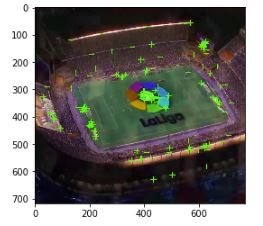
\includegraphics[width=8cm]{orb_simple_res.JPG}
\caption{Caractèristiques extraites par ORB (en vert), pour une seule image par plan}
\end{figure}

Ici, nous ne récupérons les caractèristiques que d'une seule image par plan.\\

L'algorithme est le suivant :\\
\begin{verbatim}
- Récupérer le frame à la fin de chaque shot
  - nous obtenons |S| frame
- Pour chaque frame, calculer ses features (orb ou akaze)
  - Nous obtenons |S| vecteurs
- Utiliser KMeans avec K=2 pour séparer les vecteurs en deux groupes
  - le groupe le plus petit est le groupe des logo
\end{verbatim}

\subsubsection{Première expérimentation : 1 fenêtre de frame par shot:}
\label{sec:org50a7bde}
\begin{figure}[htbp]
\centering
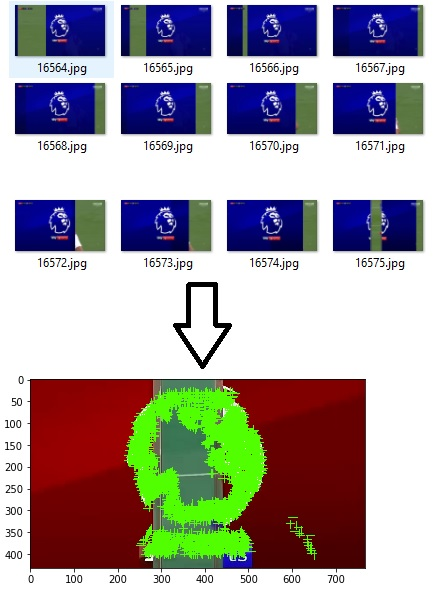
\includegraphics[width=8cm]{akaze_window_res.jpg}
\caption{Caractèristiques extraites par ORB (en vert) pour un plan (aggrégat des caractèristiques de chaque image dans le plan) \label{orb-window}}
\end{figure}
L'approche précédente ne récupère qu'une seule image par plan.\\
Or, les logos sont présents sur plusieurs frames consécutifs.\\
Dans cette approche, nous récupérons plusieurs images consécutives pour chaque plan, et nous extrayons les caractèristiques pour chaque frame (voir figure \ref{orb-window}).\\

L'algorithme est le suivant :\\
\begin{verbatim}
- Récupérer W frames pour chaque shot, les régrouper en une fenêtre
  - nous obtenons |S| fenêtres de dimension W, où W est le nombre de frame
- Pour chaque fenêtre, calculer les features de chacun de ses frames (ORB)
  - Nous obtenons un vecteur de dimension |S*W|
- Utiliser KMeans avec K=2 pour séparer les vecteurs en deux groupes
  - le groupe le plus petit est le groupe des logo
\end{verbatim}

\subsection{Analyse d'image - Seconde approche : matching de contours}
\label{sec:org86ce973}
Dans cette approche, nous allons chercher les frames qui ont des formes en commun dans la vidéo.\\
En effet, d'après l'hypothèse III, il est fort probable que si un frame à l'instant t a beaucoup de formes en commun avec un frame à l'instant t', avec \(2 < t' - t < 90\) (hypothèse V), alors il y a un logo à l'instant t et un logo à l'instant t', et un replay entre t et t'.\\

Dans cette méthode, nous utilisons là aussi le découpage en plan (\cite{Abd_Almageed_2008}) pour réduire la zone de recherche des logos de début et de fin des replays.\\

L'idée est de chercher, pour chaque plan, si il existe un autre plan dans son voisinage tel qu'ils ont des contours en commun dans plusieurs de leur frame.\\


\subsubsection{Mosaique de plan}
\label{sec:orge618fb6}
\begin{figure}[htbp]
\centering
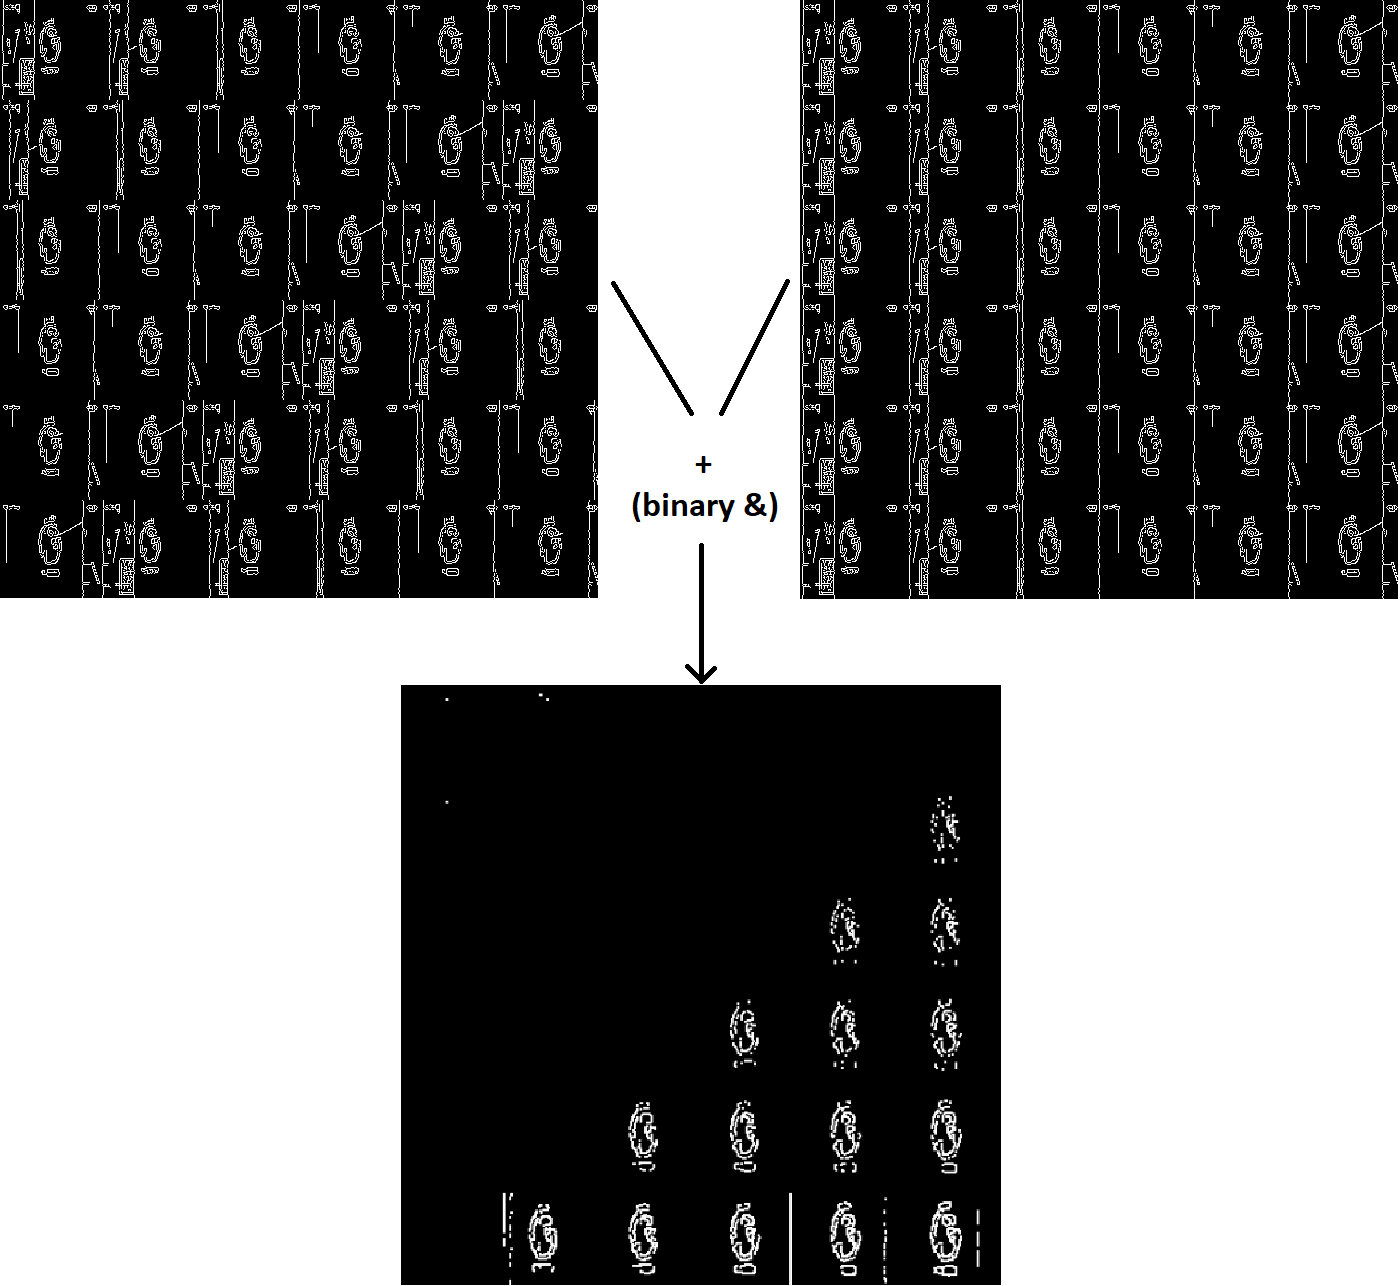
\includegraphics[width=16cm]{mosaique_add.png}
\caption{ET binaire (en bas) appliqué à une mosaique de plan à l'instant t (à gauche) et à une mosaique de plan à l'instant t' (à droite) \label{mosaic}}
\end{figure}
Pour des raisons d'optimisation, il n'est pas viable de comparer chaque frame de chaque plan avec chaque frame des plans voisins.\\

C'est pourquoi, pour chaque shot deux images sont générées.\\

Chaque image est de dimension I * I * width * height où I est le nombre de frames dans le shot.\\

Ces images sont des matrices d'images qui vont permettre de comparer rapidement deux shot.\\
La première matrice a un décalage d'un frame par ligne, la seconde n'a pas de décalage.\\

Pour comparer deux shot (figure \ref{mosaic}), il suffit d’appliquer un ET binaire entre les matrices des mosaiques, puis de calculer la longueur des contours dans cette matrice (les images sont des matrices).\\

\subsubsection{Algorithme}
\label{sec:orgc06b6b2}
\begin{verbatim}
- Pré traitement sur les shots
  1. Redimensionner
  2. Cropper
  3. Supprimer le background (s’étendre la dessus)
  4. Détecter le contour (Canny Edge Detection)
  5. Génération des mosaiques
- Pour chaque mosaique de plan S_A :
  - Pour chaque mosaique de plan S_B après S_A :
    1. Contour_commun = C_A & C_B
    2. Contours_diff = Détection du contour de Contour_commun (cv2.findContours)
    3. Résultat = Ne garder que les contours qui sont assez longs (|contours| > K)
    4. Si Résultat > Seuil : alors S_A et S_B sont des logos potentiels
- Pour chaque logo potentiel LP :
  1. Le comparer avec les autres logo L’ (même procédure qu’en 2)
  2. Si au moins 2 logo L’  match, alors LP est un logo
- Trouver les replays grâce aux logos
\end{verbatim}

Notre algorithme est sensible au plan fixe et aux images avec beaucoup de bruits (ces images ont beaucoup de contours détectés par l’algorithme de détection de contours).\\
Beaucoup de ces faux-positifs peuvent être filtrer lors du pré-traitement sur les plans, notamment en rajoutant du blur ou en supprimant le background, néanmoins, nous ne sommes pas parvenus à filtrer 100\% des faux-positifs.\\

\subsection{Apprentissage profond - Première approche : convolution 3D}
\label{sec:org81a01a1}
Dans cette approche, nous allons implémenter une méthode similaire à \cite{Tran_2015}.\\
L'idée va être d'entrainer un réseau à convolution avec une couche de convolution 3D.\\
Cette couche va prendre en entrée une séquence d'images et va prédire une classe logo ou non-logo.\\
Pour réduire la zone de recherche, seulement les séquences d'images entre deux plans (détectées avec \cite{Abd_Almageed_2008}) seront traitées.\\
Lors de l'entrainement, le réseau va apprendre à partir de séquences d'images labellisées (logo/non-logo).\\
Comme pour \cite{Tran_2015}, nous pensons que la convolution 3D va permettre au réseau d'apprendre l'apparence des logos mais aussi leur animation dans la vidéo.\\
\subsection{Apprentissage profond - Première approche : classifieur de flux optique}
\label{sec:org50d4243}
Dans cette approche, nous allons entraîner un classifieur d'image de flux optique.\\
Là aussi, nous n'allons traiter que les frames qui sont entre deux plans (\cite{Abd_Almageed_2008}).\\
Pour chaque séquence d'images comprise entre deux plans, le flux optique va être calculé pour celle-ci (entre l'image au début de la séquence et l'image à la fin de la séquence) puis une image va être générée.\\
Le réseau va apprendre à classifier les séquences en logo/non-logo à partir de ces images de flux optique.\\
\newpage
\section{Collecte des données \& entraînement}
\label{sec:org2542446}
\subsection{Datasets}
\label{sec:org531d67a}
L'objectif de la collecte de données est d'obtenir les ensembles de données suivants :\\
\begin{itemize}
\item Dataset non logo\\
\item Dataset logo\\
\end{itemize}

\subsection{Collecte des données}
\label{sec:org6fa13af}
L'approche par matching de contours convient tout à fait pour former notre ensemble de données de logo.\\

En effet, elle est :\\
\begin{itemize}
\item rapide : une vidéo au format 100x100 de 200000 frames va être traîtée en moins de cinq minutes, et en moyenne une cinquentaine de logos (séquence d'images pendant laquelle un logo apparaît) sont extraits par vidéo\\
\item précise : il est possible de modifier les paramètres pour que l'algorithme ne renvoie presque pas de faux-positifs (>1\%)\\
\end{itemize}

\subsection{Architecture du scrapper}
\label{sec:org96dd45d}
\begin{figure}[htbp]
\centering
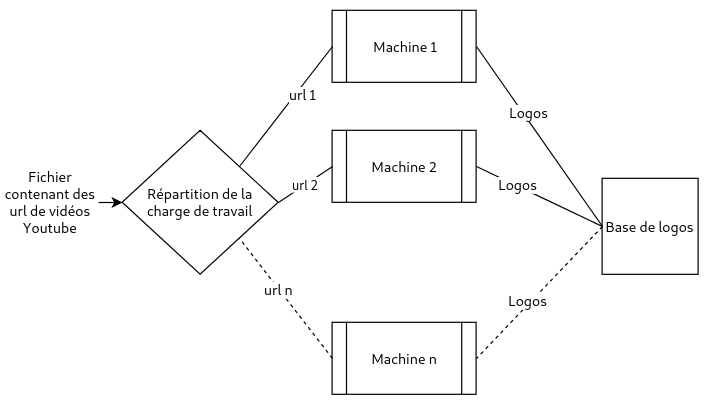
\includegraphics[width=15cm]{arch_scrap.png}
\caption{Architecture proposé pour le scrapper de logos}
\end{figure}
Nous voulons une architecture de scrapping qui soit distribuée.\\
En effet, le traitement d'une vidéo prend en moyenne cinq minutes, il est donc nécessaire de pouvoir traiter plusieurs vidéos en même temps.\\
Pour cela, nous allons créer un cluster Kubernetes qui répartira la charge de travail sur plusieurs machines.\\
Typiquement, nous utiliserons une solution type GCP (Google Cloud Platform) ou AWS (Amazon Web Services) pour l'infrastructure.\\

\newpage
\section{Comparaison des approches}
\label{sec:org469c112}
Dans cette partie, nous allons évaluer chaque approche sur le même ensemble d'évalutation.\\
Puis nous allons comparer les résultats obtenus et enfin nous allons conclure sur l'efficacité des différences approches.\\

\subsection{Procédure d'évaluation}
\label{sec:org9b694a8}
L'ensemble d'évaluation est le suivant : une vidéo de ligue 1 de 150k frames, une vidéo de ligue 1 de 80k frames, une vidéo de liga et enfin une vidéo de premier league.\\
Dans toutes les expérimentations, la vidéo est découpée en plans (plan).\\
Soit S l'ensemble des plans.\\

\subsection{Résultats pour ORB}
\label{sec:orgdb63749}
\begin{figure}[htbp]
\centering
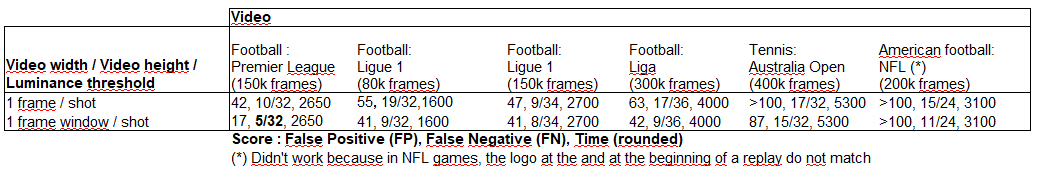
\includegraphics[width=15cm]{res_orb.png}
\caption{Résultats obtenus pour le clustering avec les caractéristiques extraites par ORB \label{orb-res}}
\end{figure}

Les résultats (\ref{orb-res}) sont mauvais sur toutes les vidéos.\\
Le gros inconvénient de ces méthodes est le caractère arbitraire de la sélection du groupe de logo après le clustering.\\
En effet, nous faisons l'hypothése qu'il y aura toujours plus de non-logo que de logo, ce qui n'est pas toujours vrai.\\
De plus, l'algorithme d'extraction de caractèristiques ne marche pas toujours très bien, ce qui fausse évidemment le clustering par la suite.\\

Néanmoins, il est intéressant de remarquer que les résultats avec la fenêtre de frame sont toujours meilleurs que les résultats avec un seul frame.\\
\subsection{Résultats pour la détection par luminance}
\label{sec:orgeb2cd95}
\begin{center}
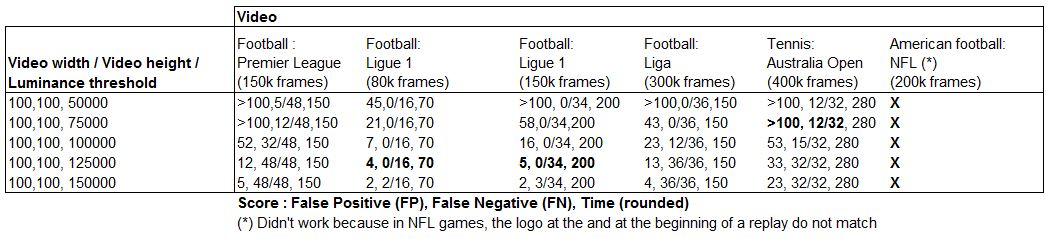
\includegraphics[width=15cm]{robust_res.JPG}
\end{center}
Après avoir implémenté la méthode de détection par luminance (\cite{xu11_robus_replay_detec_algor_soccer_video}), nous avons constaté que celle-ci n'est pas efficace et ne fonctionne pas sur notre ensemble d'évaluation.\\
Cette approche est trop dépendante de la luminance et elle ne parvient pas à détecter les logos peu lumineux.\\
De plus, les bases mathématiques (notamment la manière de choisir le cluster et la mesure de distance) sont quelque peu douteuses.\\
Enfin, celle-ci dépend trop du paramètre "seuil de luminance" affectant les logos détectés.\\
Le seuil de luminance fournis par les auteurs ne produit pas de bons résultats sur toutes les vidéos.\\
Nous n'avons pas réussi à trouver une valeur pour le seuil de luminance qui obtienne universellemnt de bons résultats.\\
Un seuil à 100000 détecte les logos de Ligue 1 mais pas les logos de Liga.\\
Un seuil de 75000 détecte les logos de Liga et de Ligue 1, mais laisse passer trop de faux positifs.\\
Les logos de Premier League quant à eux ne sont pas tous détectés avec un seuil à 50000, alors que ce seuil accepte un grand nombre de faux positifs.\\

Pour conclure, cette approche n'est pas celle qui va nous permettre de mettre en place un système de détection de replays robuste et efficace.\\

\subsubsection{Résultats pour l'approche par matching de contours}
\label{sec:orga0b201c}
\begin{figure}[htbp]
\centering
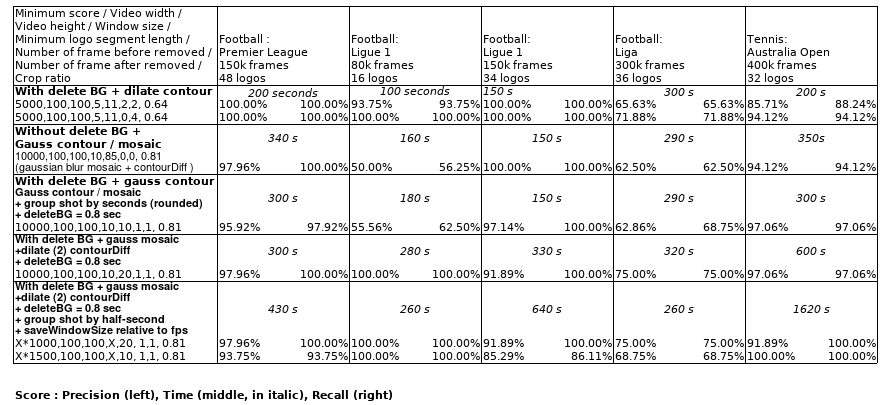
\includegraphics[width=17cm]{res_match_contour.png}
\caption{Résultats obtenus \label{res-match-contour}}
\end{figure}
Les résultats obtenus sont présentés en \ref{res-match-contour}.\\

Après avoir fait plusieurs essais avec des paramètres différents à chaque fois, nous ne sommes pas parvenus à trouver une combinaison telle qu'il n'y ait aucun faux positif et aucun faux négatif.\\
Néanmoins, si le seuil d'acceptance des logos est assez élevé, l'algorithme ne retourne aucun faux positif.\\
Ceci nous servira par la suite pour obtenir des séquences d'images logo dans les vidéos.\\

Concernant le temps d’exécution, celui-ci est relié presque entièrement à la taille de la vidéo donnée en entrée, ainsi qu’à la taille des mosaiques.\\

Les limitations de notre méthode sont les suivantes :\\
\begin{itemize}
\item Dans certaines vidéos, il n’y a pas de logo pour les replays (simple fondu)\\
\item Dans certaines vidéos, les logo de début et fin de replay ne sont pas les mêmes.\\
\item Dans certains vidéos, il y a des logo au début des replays, mais pas de logo à la fin des replays (un simple fondu remplace le logo).\\
\end{itemize}

Cette méthode présente les avantages suivants :\\
\begin{itemize}
\item elle est rapide\\
\item très peu de faux positifs\\
\end{itemize}
Néanmoins, elle n'est pas adaptative.\\
En effet, elle n'est pas capable de détecter les replays si le logo n'est pas le même au début qu'à la fin; car elle n'apprend pas ce qu'est un logo, elle sait juste trouver les images avec des contours similaires.\\

Puisque cette méthode est rapide et ne renvoie presque pas de faux positifs, elle nous servira par la suite pour créer un ensemble de données d'image avec des logo de replay.\\

Cette méthode servira aussi de \emph{baseline} pour évaluer l'efficacité des modèles par apprentissage profond.\\


\newpage
\section{Appendice}
\label{sec:orgba58bcc}
\begin{itemize}
\item Clustering : procédé permettant de regrouper des éléments\\
\item Histogramme : représentation d'une image en fonction de ses canaux de couleurs (rouge, vert, bleu)\\
\item Frame : une image à l'instant t d'une vidéo\\
\item Shot : un plan\\
\item FPS : frame per second / image par seconde\\
\item Cropper : sélectionner une partie continue des pixels l'image\\
\item RNN : Recurrent Neural Networks, ou réseaux de neurones récurrents (RNR) en français\\
\item CNN : Convolutional Neural Network, réseaux de neurones convolutifs (RNC) en français\\
\item LSTM : Long Short Term Memory\\
\end{itemize}

\newpage
\section{Table des figures}
\label{sec:orgfae6e70}
\ref{calc-dist} Xu, W., \& Yi, Y., A robust replay detection algorithm for soccer video, IEEE Signal Processing Letters, 18(9), 509–512 (2011).  \url{http://dx.doi.org/10.1109/lsp.2011.2161287}. Equation (4)\\

\ref{mean-shift-res} Duan, L., Xu, M., Tian, Q., \& Xu, C., Mean shift based video segment representation and applications to replay detection, 2004 IEEE International Conference on Acoustics, Speech, and Signal Processing, (),  ().  \url{http://dx.doi.org/10.1109/icassp.2004.1327209}. Table 1\\

\ref{sparse-vs-dense} Goodfellow, I., Bengio, Y., \& Courville, A., Deep Learning (2016), : MIT Press. \cite{Goodfellow-et-al-2016} Figure 9.2\\

\ref{optical-flow} Simonyan, K., \& Zisserman, A., Two-stream convolutional networks for action recognition in videos, CoRR, abs/1406.2199(),  (2014). Figure 2\\

\ref{c3d-res} Tran, D., Bourdev, L., Fergus, R., Torresani, L., \& Paluri, M., Learning spatiotemporal features with 3d convolutional networks, 2015 IEEE International Conference on Computer Vision (ICCV), (),  (2015).  \url{http://dx.doi.org/10.1109/iccv.2015.510}. Table 3\\

\ref{opt-flow} Simonyan, K., \& Zisserman, A., Two-stream convolutional networks for action recognition in videos, CoRR, abs/1406.2199(),  (2014). Figure 2\\

\ref{two-stream-res} Simonyan, K., \& Zisserman, A., Two-stream convolutional networks for action recognition in videos, CoRR, abs/1406.2199(),  (2014). Table 4\\

\ref{arch-c3d} Tran, D., Bourdev, L., Fergus, R., Torresani, L., \& Paluri, M., Learning spatiotemporal features with 3d convolutional networks, 2015 IEEE International Conference on Computer Vision (ICCV), (),  (2015).  \url{http://dx.doi.org/10.1109/iccv.2015.510}. Figure 3\\

\ref{arch-lstm} Ng, J. Y., Hausknecht, M., Vijayanarasimhan, S., Vinyals, O., Monga, R., \& Toderici, G., Beyond short snippets: deep networks for video classification, 2015 IEEE Conference on Computer Vision and Pattern Recognition (CVPR), (),  (2015).  \url{http://dx.doi.org/10.1109/cvpr.2015.7299101}. Figure 4\\

\ref{convolution} Goodfellow, I., Bengio, Y., \& Courville, A., Deep Learning (2016), : MIT Press. Chapitre 9. Figure 9.1\\

\ref{pooling} Goodfellow, I., Bengio, Y., \& Courville, A., Deep Learning (2016), : MIT Press. Chapitre 9. Figure 9.9\\

\ref{c3d-idea} Tran, D., Bourdev, L., Fergus, R., Torresani, L., \& Paluri, M., Learning spatiotemporal features with 3d convolutional networks, 2015 IEEE International Conference on Computer Vision (ICCV), (),  (2015).  \url{http://dx.doi.org/10.1109/iccv.2015.510}. Figure 1\\

\ref{cnn_lstm} Ng, J. Y., Hausknecht, M., Vijayanarasimhan, S., Vinyals, O., Monga, R., \& Toderici, G., Beyond short snippets: deep networks for video classification, 2015 IEEE Conference on Computer Vision and Pattern Recognition (CVPR), (),  (2015).  \url{http://dx.doi.org/10.1109/cvpr.2015.7299101}. Table 7\\
\bibliographystyle{unsrt}
\bibliography{summary}
\end{document}
